\documentclass[journal,12pt,twocolumn]{IEEEtran}
\usepackage{setspace}
\usepackage{gensymb}
\usepackage{caption}
%\usepackage{multirow}
%\usepackage{multicolumn}
%\usepackage{subcaption}
%\doublespacing
\singlespacing
\usepackage{csvsimple}
\usepackage{amsmath}
\usepackage{multicol}
%\usepackage{enumerate}
\usepackage{amssymb}
%\usepackage{graphicx}
\usepackage{newfloat}
%\usepackage{syntax}
\usepackage{listings}
%\usepackage{iithtlc}
\usepackage{color}
\usepackage{siunitx}
\usepackage{tikz}
\usetikzlibrary{shapes,arrows}
\usepackage{circuitikz}



%\usepackage{graphicx}
%\usepackage{amssymb}
%\usepackage{relsize}
%\usepackage[cmex10]{amsmath}
%\usepackage{mathtools}
%\usepackage{amsthm}
%\interdisplaylinepenalty=2500
%\savesymbol{iint}
%\usepackage{txfonts}
%\restoresymbol{TXF}{iint}
%\usepackage{wasysym}
\usepackage{amsthm}
\usepackage{mathrsfs}
\usepackage{txfonts}
\usepackage{stfloats}
\usepackage{epstopdf}
\usepackage{cite}
\usepackage{cases}
\usepackage{mathtools}
\usepackage{caption}
\usepackage{enumerate}	
\usepackage{enumitem}
\usepackage{amsmath}
%\usepackage{xtab}
\usepackage{longtable}
\usepackage{multirow}
%\usepackage{algorithm}
%\usepackage{algpseudocode}
\usepackage{enumitem}
\usepackage{mathtools}
\usepackage{hyperref}
%\usepackage[framemethod=tikz]{mdframed}
\usepackage{listings}
    %\usepackage[latin1]{inputenc}                                 %%
    \usepackage{color}                                            %%
    \usepackage{array}                                            %%
    \usepackage{longtable}                                        %%
    \usepackage{calc}                                             %%
    \usepackage{multirow}                                         %%
    \usepackage{hhline}                                           %%
    \usepackage{ifthen}                                           %%
  %optionally (for landscape tables embedded in another document): %%
    \usepackage{lscape}     


\usepackage{url}
\def\UrlBreaks{\do\/\do-}


%\usepackage{stmaryrd}


%\usepackage{wasysym}
%\newcounter{MYtempeqncnt}
\DeclareMathOperator*{\Res}{Res}
%\renewcommand{\baselinestretch}{2}
\renewcommand\thesection{\arabic{section}}
\renewcommand\thesubsection{\thesection.\arabic{subsection}}
\renewcommand\thesubsubsection{\thesubsection.\arabic{subsubsection}}

\renewcommand\thesectiondis{\arabic{section}}
\renewcommand\thesubsectiondis{\thesectiondis.\arabic{subsection}}
\renewcommand\thesubsubsectiondis{\thesubsectiondis.\arabic{subsubsection}}

% correct bad hyphenation here
\hyphenation{op-tical net-works semi-conduc-tor}

%\lstset{
%language=C,
%frame=single, 
%breaklines=true
%}

%\lstset{
	%%basicstyle=\small\ttfamily\bfseries,
	%%numberstyle=\small\ttfamily,
	%language=Octave,
	%backgroundcolor=\color{white},
	%%frame=single,
	%%keywordstyle=\bfseries,
	%%breaklines=true,
	%%showstringspaces=false,
	%%xleftmargin=-10mm,
	%%aboveskip=-1mm,
	%%belowskip=0mm
%}

%\surroundwithmdframed[width=\columnwidth]{lstlisting}
\def\inputGnumericTable{}                                 %%
\lstset{
%language=C,
frame=single, 
breaklines=true,
columns=fullflexible
}
 

\begin{document}
%
\tikzstyle{block} = [rectangle, draw,
    text width=3em, text centered, minimum height=3em]
\tikzstyle{sum} = [draw, circle, node distance=3cm]
\tikzstyle{input} = [coordinate]
\tikzstyle{output} = [coordinate]
\tikzstyle{pinstyle} = [pin edge={to-,thin,black}]

\theoremstyle{definition}
\newtheorem{theorem}{Theorem}[section]
\newtheorem{problem}{Problem}
\newtheorem{proposition}{Proposition}[section]
\newtheorem{lemma}{Lemma}[section]
\newtheorem{corollary}[theorem]{Corollary}
\newtheorem{example}{Example}[section]
\newtheorem{definition}{Definition}[section]
%\newtheorem{algorithm}{Algorithm}[section]
%\newtheorem{cor}{Corollary}
\newcommand{\BEQA}{\begin{eqnarray}}
\newcommand{\EEQA}{\end{eqnarray}}
\newcommand{\define}{\stackrel{\triangle}{=}}
\bibliographystyle{IEEEtran}
%\bibliographystyle{ieeetr}
\providecommand{\nCr}[2]{\,^{#1}C_{#2}} % nCr
\providecommand{\nPr}[2]{\,^{#1}P_{#2}} % nPr
\providecommand{\mbf}{\mathbf}
\providecommand{\pr}[1]{\ensuremath{\Pr\left(#1\right)}}
\providecommand{\qfunc}[1]{\ensuremath{Q\left(#1\right)}}
\providecommand{\sbrak}[1]{\ensuremath{{}\left[#1\right]}}
\providecommand{\lsbrak}[1]{\ensuremath{{}\left[#1\right.}}
\providecommand{\rsbrak}[1]{\ensuremath{{}\left.#1\right]}}
\providecommand{\brak}[1]{\ensuremath{\left(#1\right)}}
\providecommand{\lbrak}[1]{\ensuremath{\left(#1\right.}}
\providecommand{\rbrak}[1]{\ensuremath{\left.#1\right)}}
\providecommand{\cbrak}[1]{\ensuremath{\left\{#1\right\}}}
\providecommand{\lcbrak}[1]{\ensuremath{\left\{#1\right.}}
\providecommand{\rcbrak}[1]{\ensuremath{\left.#1\right\}}}
\theoremstyle{remark}
\newtheorem{rem}{Remark}
\newcommand{\sgn}{\mathop{\mathrm{sgn}}}
%\providecommand{\abs}[1]{\left\vert#1\right\vert}
\providecommand{\res}[1]{\Res\displaylimits_{#1}} 
\providecommand{\norm}[1]{\lVert#1\rVert}
\providecommand{\mtx}[1]{\mathbf{#1}}
%\providecommand{\mean}[1]{E\left[ #1 \right]}
\providecommand{\fourier}{\overset{\mathcal{F}}{ \rightleftharpoons}}
%\providecommand{\hilbert}{\overset{\mathcal{H}}{ \rightleftharpoons}}
\providecommand{\system}{\overset{\mathcal{H}}{ \longleftrightarrow}}
	%\newcommand{\solution}[2]{\textbf{Solution:}{#1}}
\newcommand{\solution}{\noindent \textbf{Solution: }}
\newcommand{\myvec}[1]{\ensuremath{\begin{pmatrix}#1\end{pmatrix}}}
\providecommand{\dec}[2]{\ensuremath{\overset{#1}{\underset{#2}{\gtrless}}}}
\DeclarePairedDelimiter{\ceil}{\lceil}{\rceil}
%\numberwithin{equation}{section}
%\numberwithin{problem}{subsection}
%\numberwithin{definition}{subsection}
\makeatletter
\@addtoreset{figure}{section}
\makeatother
\let\StandardTheFigure\thefigure
%\renewcommand{\thefigure}{\theproblem.\arabic{figure}}
\renewcommand{\thefigure}{\thesection}
%\numberwithin{figure}{subsection}
%\numberwithin{equation}{subsection}
%\numberwithin{equation}{section}
%\numberwithin{equation}{problem}
%\numberwithin{problem}{subsection}
\numberwithin{problem}{section}
%%\numberwithin{definition}{subsection}
%\makeatletter
%\@addtoreset{figure}{problem}
%\makeatother
\makeatletter
\@addtoreset{table}{section}
\makeatother
\let\StandardTheFigure\thefigure
\let\StandardTheTable\thetable
\let\vec\mathbf
%%\renewcommand{\thefigure}{\theproblem.\arabic{figure}}
%\renewcommand{\thefigure}{\theproblem}
%%\numberwithin{figure}{section}
%%\numberwithin{figure}{subsection}
\def\putbox#1#2#3{\makebox[0in][l]{\makebox[#1][l]{}\raisebox{\baselineskip}[0in][0in]{\raisebox{#2}[0in][0in]{#3}}}}
     \def\rightbox#1{\makebox[0in][r]{#1}}
     \def\centbox#1{\makebox[0in]{#1}}
     \def\topbox#1{\raisebox{-\baselineskip}[0in][0in]{#1}}
     \def\midbox#1{\raisebox{-0.5\baselineskip}[0in][0in]{#1}}
\vspace{3cm}
\title{ 
%	\logo{
Gain Analysis for LM386 Audio Amplifer 
%	}
}
\author{ Nachiket Chouhan and N. Dileep Chandra $^{*}$% <-this % stops a space
	\thanks{*The author is with the Department
		of Electrical Engineering, Indian Institute of Technology, Hyderabad
		502285 India e-mail:  gadepall@iith.ac.in. All solutions in this manual is released under GNU 
GPL.  Free and open source.}
	
}
\maketitle
\tableofcontents
\bigskip
\renewcommand{\thefigure}{\theenumi}
\renewcommand{\thetable}{\theenumi}
\begin{abstract}
This manual provides the gain analysis for the LM386 audio amplifier. 
\end{abstract}

\section{Equivalent Circuit of LM386}
%\begin{enumerate}[label=\arabic*]
\begin{enumerate}[label=\thesection.\arabic*,ref=\thesection.\theenumi]
\numberwithin{equation}{enumi}
%\begin{figure}[!ht]
%\centering
%\includegraphics[width=\columnwidth]{LM386int.eps}
%\caption{}
%\label{fig:1}
%\end{figure}

\begin{figure}[!ht]
%\begin{center}
\centering	
%\includegraphics[width=\columnwidth]{./figs/right_angle_tri.tex}
\resizebox{\columnwidth}{!}{%\documentclass{article}
%\usepackage{siunitx}
%\usepackage{tikz}
%\usepackage{circuitikz}
%\usepackage[export]{adjustbox}
%
%\begin{document}
%
%\begin{figure}

    \begin{circuitikz}[american]
    
  \draw (0,0) node(anchor=west){Q3};  
  \draw (0,0) node[pnp](pnp3) {}                %Q3
  (pnp3.base) node[] {}
  (pnp3.collector) node[] {}
  (pnp3.emitter) node[] {};
  \draw (pnp3.emitter) to[R=\SI{15}{\kohm}] ++(0,2.5)
  to[R=\SI{15}{\kohm}] ++(0,2.5);
  
  \draw ((-1,-1) node(anchor=west){Q1};  
  \draw (-1,-1) node[pnp](pnp1) {}                %Q1
  (pnp1.base) node[] {}
  (pnp1.collector) node[] {}
  (pnp1.emitter) node[] {};
  
  \draw (pnp3.base) to[short] (pnp1.emitter);
  \filldraw [black] (-1.84,-1) circle (2pt);
  \draw (pnp1.base) to[R=\SI{50}{\kohm}] ++(0,-4);
  \draw (pnp1.base) to[short] ++(-0.7,0)
  to [black] (-3,-1) circle (2pt); 
  \draw (-3,-1.3) node(anchor=west){-input};
       \draw (-3,-0.7) node(anchor=north){2};                           %2 -input
  \draw (-1.84,-5) to[short] (12,-5);
  \draw (pnp3.emitter) to[R=\SI{150}{\ohm}] ++(2,0)
  to[R=\SI{1.35}{\kohm}] ++(2,0);
  \draw (0,5.77) to[short] (12,5.77);
  \draw [black] (12,5.77) circle (2pt);
   \draw (12.1,5.47) node(anchor=west){supply};
   \draw (12,6) node(anchor=north){6};                      %6 supply
  \draw [black] (12,-5) circle (2pt); 
  \draw (12.1,-5.3) node(anchor=west){ground};
   \draw (12,-4.7) node(anchor=north){4};                      %4 ground
  \filldraw [black] (4,0.77) circle (2pt);
  \draw (4,0.77) to[short] (4,1.9);
  \draw [black] (4,1.96) circle (2pt); 
  \draw (4,2.2) node(anchor=west){8};
   \draw (4,2.5) node(anchor=north){gain};                   %8 gain
    \filldraw [black] (2,0.77) circle (2pt);
    \draw (2,0.77) to[short] (2,1.9);
    \draw [black] (2,1.96) circle (2pt); 
    \draw (2,2.2) node(anchor=west){1};
   \draw (2,2.5) node(anchor=north){gain};                  %1 gain
  \filldraw [black] (0,3.5) circle (2pt);
  \draw (0,3.5) to[short] (-1,3.5);
  \draw [black] (-1,3.5) circle (2pt); 
  \draw (-1,3.2) node(anchor=west){bypass};
       \draw (-1,3.8) node(anchor=north){7};                       %7 bypass
  \draw (pnp1.collector) to[short] (-1,-5);
  \filldraw [black] (0,0.77) circle (2pt);
  \filldraw [black] (-1,-5) circle (2pt);    
   \filldraw [black] (0,-5) circle (2pt); 
   
  \draw (0,-4.25) node(anchor=west){Q5};    
   \draw (0,-4.25) node[npn, xscale=-1](npn5){}   %5
  (npn5.base) node[] {}
  (npn5.collector) node[] {}
  (npn5.emitter) node[] {};
  
   \draw (pnp3.collector) to[short] (npn5.collector);
   \draw (npn5.base) to[short] (0.84,-3.47);
   \draw (npn5.collector) to[short] (0.84,-3.47);
   \filldraw [black] (npn5.collector) circle (2pt); 
   \filldraw [black] (npn5.base) circle (2pt); 
   
     \draw (4,0) node(anchor=west){Q4};  
\draw (4,0) node[pnp, xscale=-1](pnp4){}   %4
  (pnp4.base) node[] {}
  (pnp4.collector) node[] {}
  (pnp4.emitter) node[] {};
  
    \draw (4,-4.25) node(anchor=west){Q6};  
\draw (4,-4.25) node[npn](npn6){}   %6
  (npn6.base) node[] {}
  (npn6.collector) node[] {}
  (npn6.emitter) node[] {};
  
   \draw (pnp4.collector) to[short] (npn6.collector);
   \draw (npn5.base) to[short] (npn6.base);
     \filldraw [black] (npn6.emitter) circle (2pt); 
     \filldraw [black] (npn6.collector) circle (2pt); 
     
      \draw (5,-1) node(anchor=west){Q2};  
   \draw (5,-1) node[pnp, xscale=-1](pnp2){}   %2
  (pnp2.base) node[] {}
  (pnp2.collector) node[] {}
  (pnp2.emitter) node[] {};  
  
  \draw (pnp2.base) to[short] ++(1,0)
  to [black] (7,-1) circle (2pt); 
  \draw (7,-0.7) node(anchor=west){3};
   \draw (7,-1.3) node(anchor=north){+Input};                            %3 input
  \draw (pnp4.base) to[short] (pnp2.emitter); 
  \draw (5,-5) to[short] (pnp2.collector);
  
      \draw (9,-3.47) node(anchor=west){Q10};  
\draw (9,-3.47) node[npn](npn10){}   %10
  (npn10.base) node[] {}
  (npn10.collector) node[] {}
  (npn10.emitter) node[] {};
  
  \filldraw [black] (pnp2.base) circle (2pt); 
  
  \draw (npn6.collector) to[short] (npn10.base); 
    \draw (pnp2.base) to[R=\SI{50}{\kohm}] ++(0,-4);
    
    \draw (pnp4.emitter) to[R=\SI{15}{\kohm}] ++(5,0)
    to[diode] (9,-1)
    to[short] (npn10.collector);
    \draw (6.5,1.6) node(anchor=north){$R_f$};
   \draw (npn10.emitter) to[short] (9,-5);
   \filldraw [black] (9,-5) circle (2pt); 
  
        \draw (9.85,-1.5) node(anchor=west){Q8};  
\draw (9.85,-1.5) node[pnp](pnp8) {}       %Q8
  (pnp8.base) node[] {}
  (pnp8.collector) node[] {}
  (pnp8.emitter) node[] {};
  
\draw (pnp8.emitter) to[short] ++(1.15,0);
   \filldraw [black] (pnp8.base) circle (2pt);
    \filldraw [black] (9,5.77) circle (2pt);
\draw (9,5.77) to[I, i_=$.$] (9,3);               %current sourse
    \draw (9,3) to[diode] (9,0.77);
    
     \draw (11,3) node(anchor=west){Q7};  
   \draw (11,3) node[npn](npn7){}   %7
  (npn7.base) node[] {}
  (npn7.collector) node[] {}
  (npn7.emitter) node[] {};
  
  \draw (npn7.base) to[short] (9,3);
    \draw (npn7.collector) to[short] (11,5.77);
   \draw (9,0.77) to[short] (12,0.77);
   
   \draw (11,-4.23) node(anchor=east){Q9};  
  \draw (11,-4.23) node[npn](npn9){}   %9
  (npn9.base) node[] {}
  (npn9.collector) node[] {}
  (npn9.emitter) node[] {};
   
   \filldraw [black] (npn9.emitter) circle (2pt);
  \draw (pnp8.collector) to[short] (npn9.base);
    \draw (npn7.emitter) to[short] (npn9.collector);
   \filldraw [black] (npn9.emitter) circle (2pt);
  \filldraw [black] (11,0.77) circle (2pt);
  \filldraw [black] (11,-0.73) circle (2pt);
  \draw [black] (12,0.77) circle (2pt);
  \draw (12.1,0.47) node(anchor=west){output};
   \draw (12,1) node(anchor=north){5};                   %5 output
   
   
   \draw (0.5,0.2) to[short] (3.5,0.2);
   \draw (0.5,0.2) to[short] (0.5,0.3);
  \draw (3.5,0.2) to[short] (3.5,0.3);
   \draw (2,-0.1) node(anchor=north){$R_e$}; 
   
    
     \draw (2,-3.2) node(anchor=north){Current};  
   \draw (2,-3.5) node(anchor=north){mirror};
   \draw [dashed] (-0.3,-3) -- (4.4,-3);
   \draw [dashed] (-0.3,-3) -- (-0.3,-5.4);
   \draw [dashed] (-0.3,-5.4) -- (4.4,-5.4);
   \draw [dashed] (4.4,-5.4) -- (4.4,-3);
   


   \end{circuitikz}  
   
%\end{figure}
%
%\end{document}
}
%\vspace*{-10cm}
%\end{center}
\caption{LM386 Amplifier}
\label{fig:orig}	
\end{figure}


\section{ Common Collector(Emitter Follower) Buffer}

\numberwithin{equation}{enumi}

\item What is the gain of Common collector transistor amplifier?\\
\solution 
The voltage gain of amplifier in CC state is a little less than 1.
\begin{figure}[!ht]
\centering	
\resizebox{\columnwidth}{!}{%\documentclass{article}
%\usepackage[absolute,overlay]{textpos}
%\usepackage{tikz}
%\usepackage{circuitikz}
%\usepackage[absolute]{textpos}
%
%
%\begin{document}
%
%
%\begin{figure}[h!]
\begin{circuitikz}
  \draw (0,0) node[pnp](pnp1) {}
  (pnp1.base) node[] {}
  (pnp1.collector) node[] {}
  (pnp1.emitter) node[] {};
  \draw (-0.15,0) circle [radius=15pt];
  \draw (pnp1.emitter) to[R=$R_c$] ++(0,2)
  to[short] (4,2.77);
  \draw (pnp1.collector) to[short] (0,-2)
  to[short] (4,-2);
  
   \draw (4,2.77) to [battery={$V_{\mathrm{EC}}$}] (4,-2); 
  \draw (pnp1.base) to[short] (-3,0)
  to[short] (-3,-0.7);

  \draw (-3,-1.3) to[short] (-3,-2);
  
\draw (0,-2) to [battery={$V_{\mathrm{BC}}$}] (-3,-2);    %{t_{\mathrm{max}}} 
  
  \draw (pnp1.collector) to[short] (1,-0.77);
  \draw (1,-0.77) circle [radius=2pt];
  \draw [arrows=<->] (1,-0.68) -- (1,2.74);
  \draw (1.6,1) node(anchor=north){Output};
  \draw (-3,-1) node(anchor=north){signal};  
  
  \end{circuitikz}

%\end{figure}
%
%
%\end{document}
}
\caption{Common Collector Amplifier}
\label{fig:cc}	
\end{figure}

\item What is the use of Q1 and Q2 in the internal circuit?\\
\solution
The first block is a PNP Emitter Follower amplifier (Q1, Q2), it sets the input impedance and defines the DC operation points, raising the input voltages off the ground so the circuit will accept negative input signal down to -0.4 V. Both 50k input resistors (R1, R3) create the path to ground of the base current, the input needs to be coupled so not to disturb the internal biasing, hence the input impedance is dominated by these resistors and set to 50K.
%
\begin{figure}[!ht]
\centering	
\resizebox{\columnwidth}{!}{%\documentclass{article}
%\usepackage{siunitx}
%\usepackage{tikz}
%\usepackage{circuitikz}
%
%\begin{document}
%\begin{figure}[h!]
\begin{circuitikz}

%left side part
  \draw (-1,0) node[pnp](pnp1){}            %Q3
  (pnp1.base) node[] {}
  (pnp1.collector) node[] {}
  (pnp1.emitter) node[] {};
  \draw (-1,0) node(anchor=east){Q3};
  \draw (pnp1.base) to[short] (-1.85,-0.5);
  \draw (-1.85,-.79) node[pnp](pnp2) {}                  %Q1
  (pnp2.base) node[] {}
  (pnp2.collector) node[] {}
  (pnp2.emitter) node[] {};
  \draw (-1.85,-0.79) node(anchor=east){Q1};
  \draw (pnp2.base) to[short] (-3.9,-0.79);
  \draw (-3.4,-.78) to[R=\SI{50}{\kohm}] (-3.4,-2.5)
  to[short] (-1.85,-2.5)
  to[short] (-1.85,-1.5);
  \filldraw [black] (-2.5,-2.5) circle (2pt);
  \filldraw [black] (-3.4,-.78) circle (2pt);
  \draw [black] (-3.95,-.78) circle (2pt);
  \draw (-4.6,-.78) node(anchor=east){-Input};                     %-input
  \draw (-2.5,-2.5) to[short] (-2.5,-2.9);
  \draw (-2.2,-2.9) to[short] (-2.8,-2.9);
  \draw (-2.2,-2.9) to[short] (-2.5,-3.3);
  \draw (-2.8,-2.9) to[short] (-2.5,-3.3);
  
%right side part
  \draw (1,0) node[pnp, xscale=-1](pnp3){}                     %Q4
  (pnp3.base) node[] {}
  (pnp3.collector) node[] {}
  (pnp3.emitter) node[] {};
  \draw (1,0) node(anchor=east){Q4};
  \draw (pnp3.base) to[short] (1.85,-0.5);
  \draw (1.85,-.79) node[pnp,xscale=-1](pnp4){}            %Q2
  (pnp4.base) node[] {}
  (pnp4.collector) node[] {}
  (pnp4.emitter) node[] {};
  \draw (1.85,-0.79) node(anchor=east){Q2};
  \draw (pnp4.base) to[short] (3.9,-0.79);
  \draw (3.4,-.78) to[R=\SI{50}{\kohm}] (3.4,-2.5)
  to[short] (1.85,-2.5)
  to[short] (1.85,-1.5);
  \filldraw [black] (2.5,-2.5) circle (2pt);
  \filldraw [black] (3.4,-.78) circle (2pt);
  \draw [black] (3.95,-.78) circle (2pt);  
  \draw (4.7,-.78) node(anchor=east){+Input};                      %+input
  \draw (2.5,-2.5) to[short] (2.5,-2.9);
  \draw (2.2,-2.9) to[short] (2.8,-2.9);
  \draw (2.2,-2.9) to[short] (2.5,-3.3);
  \draw (2.8,-2.9) to[short] (2.5,-3.3);  
  
  \draw (pnp1.emitter) node(anchor=east)[xshift=-3]{//};
  \draw (pnp1.collector) node(anchor=east)[xshift=3]{//};
  \draw (pnp3.emitter) node(anchor=east)[xshift=-3]{//};
  \draw (pnp3.collector) node(anchor=east)[xshift=3]{//};
  
  
  
  
\end{circuitikz}
%\end{figure}
%\end{document}
}
\caption{Common Collector-Differential Amplifier}
\label{fig:ccdiff}	
\end{figure}
\end{enumerate}


\section{Differential amplifier}
\begin{enumerate}[label=\thesection.\arabic*,ref=\thesection.\theenumi]
\numberwithin{equation}{enumi}
\item What is a differential amplifier?\\
\solution The differential amplifier can be considered as an analog circuit which consists of two inputs and one output. The differential amplifier circuit can be represented as shown in the figure below.\\
\item What is the output of a differential amplifier?\\
\solution The output voltage of a differential amplifier is proportional to the difference between the two input voltages. This can be represented in equation form as follows:
Differential Amplifier Gain $$G = A(V_{b3}-V_{b4})$$
where $V_{b3}$ and $V_{b3}$ are input base voltages to Q3 and Q4 of differential amplifier and A is the gain of individual amplifiers,assuming them to be identical.\\


\item What is the output of the differential amplifier in the above circuit?\\

 \solution The gain is 1 in this case because voltage drop across base-emitter of transistors Q1,Q2,Q3 ad Q4 is same and all are CC transistors.Therefoere, the voltage drop across $R_{e}$ will be same as difference between the input voltages.\\\textit{(Note :Section 1 we mentioned gain of CC transistor amplifier is almost 1.)}\\
\begin{figure}[!ht]
\centering	
\resizebox{\columnwidth}{!}{%\documentclass{article}
%\usepackage{siunitx}
%\usepackage{tikz}
%\usepackage{circuitikz}
%
%\begin{document}
%
%\begin{figure}[h!]
%  \begin{center}
    \begin{circuitikz}
      
    
  \draw (-2,-1) node[pnp](pnp1){}
  (pnp1.base) node[] {}
  (pnp1.collector) node[] {}
  (pnp1.emitter) node[] {};
  \draw (-1.9,-1) node(anchor=east){Q3};
  
  \draw (pnp1.emitter) to[short] (-2,0)
  to[R=\SI{150}{\ohm}] (0,0);
  \draw (-2,0) to[short] (-2,1);
  \draw [black] (0,1.06) circle (2pt);
  \draw (0,1.3) node(anchor=east){8};
  
  
  \draw (2,-1) node[pnp, xscale=-1](pnp2){}
  (pnp2.base) node[] {}
  (pnp2.collector) node[] {}
  (pnp2.emitter) node[] {};
  \draw (1.9,-1) node(anchor=east){Q4};
  
  \draw (pnp2.emitter) to[short] (2,0)
  to[R=\SI{1.35}{\kohm}, yscale=-3] (0,0);
  \draw (2,0) to[short] (2,1);
  \draw [black] (2,1.06) circle (2pt);
  \draw (2,1.3) node(anchor=east){1};
  \draw (2,0) to[short] (3,0);
  \draw (0,0) to[short] (0,1);
  
  \filldraw [black] (0,0) circle (2pt); 
  \filldraw [black] (2,0) circle (2pt); 
  \filldraw [black] (-2,0) circle (2pt);
  
  \draw (-2,1) node(anchor=east)[xshift=-3]{//};
  \draw (3,0) node(anchor=east)[xshift=3]{//};
  \draw (pnp2.base) node(anchor=east)[xshift=3]{//};
  \draw (pnp2.collector) node(anchor=east)[xshift=3]{//};
  \draw (pnp1.base) node(anchor=east)[xshift=-3]{//};
  \draw (pnp1.collector) node(anchor=east)[xshift=3]{//};
  
  \draw (-1.8,-0.5) to[short] (1.8,-0.5);
   \draw (-1.8,-0.5) to[short] (-1.8,-0.3);
  \draw (1.8,-0.3) to[short] (1.8,-0.5);
   \draw (0,-0.8) node(anchor=north){$R_e$}; 

   \end{circuitikz}
%  \end{center}
%\end{figure}
%
%\end{document}
}
\caption{Differential Amplifier}
\label{fig:diff}	
\end{figure}
\end{enumerate}
% \begin{figure}[!ht]
%\centering
%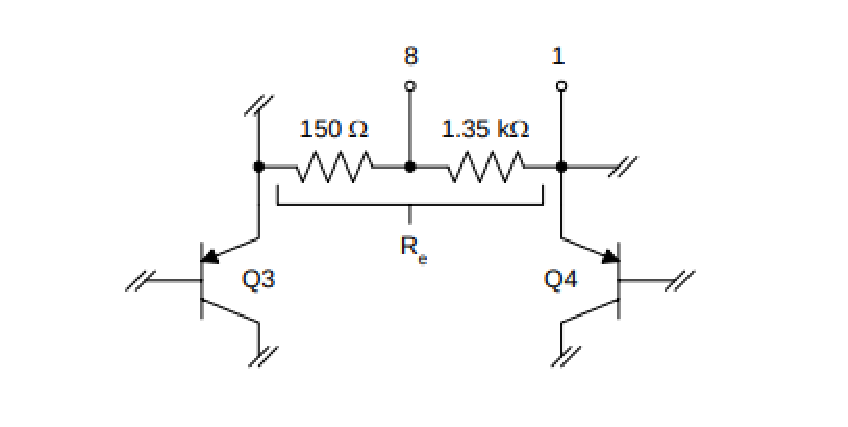
\includegraphics[width=0.7\columnwidth]{./figs/LM3662.eps}
%\caption{}
%\label{fig:1}
%\end{figure}

%\end{enumerate}

\section{Current Mirror}
\begin{enumerate}[label=\thesection.\arabic*,ref=\thesection.\theenumi]
\item What is a Current mirror?\\
\solution Current mirror circuits generally consist two main transistor, although other devices such as FETs can be used. The current mirror circuit gains its name because it copies or mirrors the current flowing in one active device in another, keeping the output current constant regardless of loading.
\item Comment about how the current mirror works in the IC.\\
\solution
Q5 and Q6 form a current mirror.The differential amplifier is biased by the current mirror.A current mirror is a circuit block which functions to produce a copy of the current flowing into or out of an input terminal by replicating the current in an output terminal.\\
This can be proved by,
\bigskip
\vspace{-1em}
$$V_{be(Q5)}=V_{be(Q6)}=V_b$$\\
\vspace{-1em}
$$I_c=I_{cs}e^{V_b/V_t}$$\\
\vspace{-1em}
$$I_{c5}=I_{c6}$$\\
\vspace{-0.5em}
Since the two transistors are matched,\\
\vspace{-1em}
$$I_{E5}=I_{E6}$$\\
\vspace{-0.5em}
Neglecting the base currents by assuming large $\beta$ .\\
\vspace{-1em}
$$I_5=I_6$$

\begin{figure}[!ht]
\centering	
\resizebox{\columnwidth}{!}{%\documentclass{article}
%\usepackage{siunitx}
%\usepackage{tikz}
%\usepackage{circuitikz}
%\usepackage[utf8]{inputenc}
%\usepackage{amsmath}
\newcommand{\approxtext}[1]{\ensuremath{\stackrel{\text{#1}}{\approx}}}

%\begin{document}
%  \begin{figure}[h!]
    \begin{circuitikz} 

\draw (-.84,0) node[npn, xscale=-1](npn5){}                     %Q6
  (npn5.base) node[] {}
  (npn5.collector) node[] {c}
  (npn5.emitter) node[] {};
  
\draw (.84,0) node[npn](npn6){}                     %Q5
  (npn6.base) node[] {}
  (npn6.collector) node[] {c}
  (npn6.emitter) node[] {};  
  
\draw (npn6.emitter) to[short] (npn5.emitter);  
\draw (npn5.collector) to[short] (0,0.77);  
\draw (npn5.base) to[short] (0,0.77);

\draw (0,-1) to[short] (0,-0.77);
\draw (0.25,-1) to[short] (-0.25,-1);
\draw (0.25,-1) to[short] (0,-1.4);
\draw (0,-1.4) to[short] (-0.25,-1);

\draw (0.84,2) to[short] (npn6.collector);
\draw (-0.84,2) to[short] (npn5.collector);
  
\draw (0.84,2) node(anchor=east)[xshift=-3]{//};
\draw (-0.84,2) node(anchor=east)[xshift=-3]{//};  
  
\draw (0.85,0) node(anchor=east){Q6};  
\draw (-0.85,0) node(anchor=east){Q5}; 

\draw (-0.1,-0.1) node(anchor=east){\tiny +};
\draw (-0.1,-0.67) node(anchor=east){\tiny -};   
\draw (-0.1,-0.4) node(anchor=east){\scriptsize $V_b$};  
  
\draw [arrows=->] (0.84,1.6) -- (0.84,1.2);
\draw [arrows=->] (-0.84,1.6) -- (-0.84,1.2); 
\draw [arrows=->] (-0.5,0.77) -- (-0.2,0.77);
  
\draw (-1,1.42) node(anchor=east){\scriptsize $I_5$};
\draw (1,1.42) node(anchor=east){\scriptsize $I_6$};  
\draw (-0.2,1) node(anchor=east){\scriptsize I \approxtext{} 0};  
  
\filldraw [black] (npn5.base) circle (2pt);  
\filldraw [black] (npn5.collector) circle (2pt);
\filldraw [black] (0,-0.77) circle (2pt);
  
    \end{circuitikz}
%  \end{figure}
%\end{document}
}
\caption{Current Mirror}
\label{fig:cmirror}	
\end{figure}

% \begin{figure}[!ht]
%\centering
%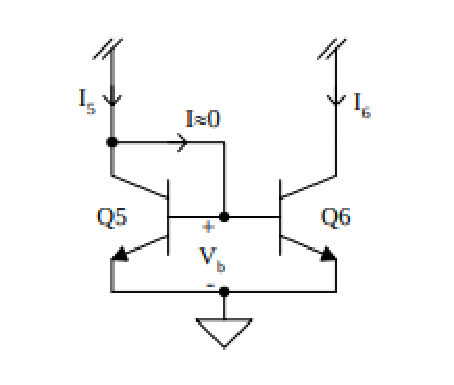
\includegraphics[width=0.7\columnwidth]{./figs/LM3863.eps}
%\caption{}
%\label{fig:1}
%\end{figure}

\end{enumerate}





\section{Small Signal Analysis}
\begin{enumerate}[label=\thesection.\arabic*,ref=\thesection.\theenumi]
\item Draw the small signal equivalent of the internal circuit excluding the BJTs.\\

\solution Fig. 5.1

\begin{figure}[!ht]
\centering	
\resizebox{\columnwidth}{!}{%\documentclass{article}
%
%\usepackage{tikz}
%\usepackage{circuitikz}
%\usepackage{siunitx}
%
%\begin{document}
%
%\begin{figure}
%  \begin{center}
    \begin{circuitikz}
      \draw (0,0)
      to[R=$\SI{15}{\kilo\ohm}$,i_=$\approx$0,o-o] (0,2) % The voltage source
      to[R=$\SI{15}{\kilo\ohm}$,o-.] (0,4)
      to[short] (1,4) node[sground]{}
      (0,2) to [short,o-o] (-1,2)node[anchor=east] {7}
      (2,-0.5) node[anchor=north] {-$v_d$+}
      (0,0)to[R=$R_e$,o-o](4,0)
       (6,0)to[R=$R_f$,i_=$\approx$2i,o-.] (4,0)
      (6,0)node[anchor=west] {$v$}
      (0,0) to [short,i_=i,o-o] (0,-1) 
      (4,0) to [short,i_=i,o-o] (4,-1)
      (0,0) to [short] (-1,0) node[sground]{}
      (-1,-0.2) circle (0.5) (-1,0.5)node[anchor=east] {$\approx$}
      (2,-1) node[anchor=north] {Equal because of}
      (2,-1.5) node[anchor=north] {current mirror};
      
    \end{circuitikz}
   
%  \end{center}
%\end{figure}
%
%\end{document}
}
\caption{Current Mirror: Small Signal Analysis}
\label{fig:smallsig}	
\end{figure}
%\begin{figure}[!ht]
%\centering
%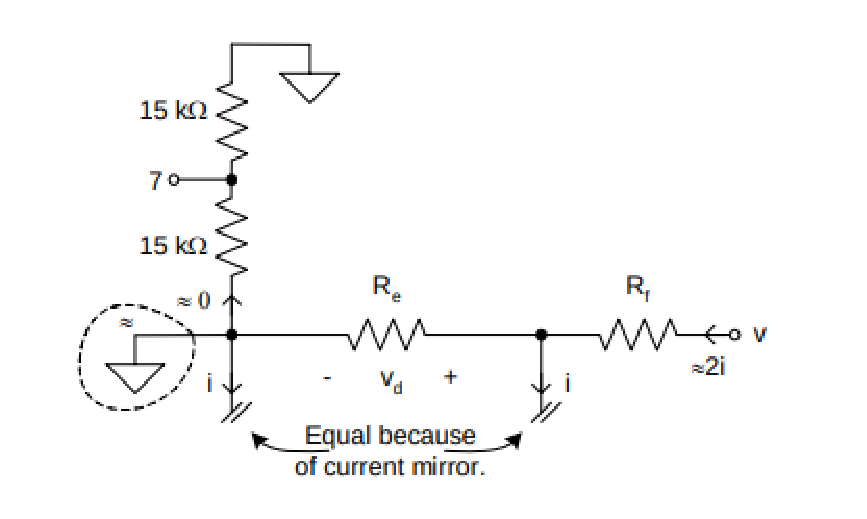
\includegraphics[width=0.7\columnwidth]{./figs/LM3866.eps}
%\caption{}
%\label{fig:2}
%\end{figure}

\item Derive the relation between input voltage(across differential amplifier) and output voltage.\\
\solution
The current mirror forces the currents on both halves of the
differential amplifier to be equal: both dc and ac components.\\
Consequently, the currents i at the emitters of Q3 and Q4 must
be the same, as shown in Fig.5.6.\\ Due to the mirror, the current through $R_{f} = 2 i$(approx) , neglecting the current in the two $15k\ohm$ resistors (which are large impedances
relative to the other parts of the circuit). Therefore,\\
$$\frac{v-v_{d}}{R_{f}}=2i$$   

\item Given the class AB amplifier what will be the $\beta$ for the compund pnp transistor in terms of individual $\beta$?

\begin{figure}[!ht]
\centering	
\resizebox{\columnwidth}{!}{%\documentclass{article}
%
%\usepackage{tikz}
%\usepackage{circuitikz}
%\usepackage{siunitx}
\usetikzlibrary{calc}
%\ctikzset{bipoles/thickness=1}
%\ctikzset{bipoles/length=0.8cm}
\ctikzset{bipoles/diode/height=.3}
\ctikzset{bipoles/diode/width=.2}
%\begin{document}

%\begin{figure}
%  \begin{center}
    \begin{circuitikz}[american currents]
    \draw
    (0,0) node[pnp] (pnp){}
    (2,-2) node[npn] (npn1){}
    (-0.8,-2) node[npn] (npn2){}
    %(-0.8,2) to[full diode] (d1) (-0.8,1)
    (pnp.C) to [short] (0,-2)to [short] (npn1.B)
    (npn1.C) to [short] (2,0.8)
    (pnp.E) to [short] (2,0.8)   (2,1)to [short] (2,0.8)node[anchor =west] {$i_e$}
    (npn2.E) to [short,*-*] (npn1.E) to [short,-o] (2.5,-2.8) node[anchor =west] {Gnd}
    (npn2.C) to [short,-*] (pnp.B) 
     (-0.85,1)to[full diode](pnp.B) 
        (-0.85,1)to[short] (-0.85,2) 
            to[full diode]  (-0.85,1) to [short,-*] (-0.85,2.5)
            (-0.85,4.5) to [I,*-*] (-0.85,2.5) to [short] (1.15,2.5) (2,2.5) node[npn] (npn3){} (npn3.E) to [short] (2,1)
    %(d1.n) to [short] (pnp.B)
  (-0.85,1)to [short] (-2,1)  to [R =$R_f$](-3.5,1) node[anchor =east] {//}
  (-0.85,1)to[short,-*] (2,1) to [short,-o] (3,1)node[anchor =west] {Out}
  node[anchor =north] {$v$} node[anchor =south] {5}
  (npn3.C) to [short,-*] (2,4.5) to[short] (-0.85,4.5)to[short](-3.5,4.5)node[anchor =east] {//}
  (2,4.5) to [short,-o] (3,4.5)node[anchor =west] {$V_{cc}$}node[anchor =south] {6}
  (npn2.B)to [short] (-3.5,-2) node[anchor =east] {//}
    (npn2.E)to [short] (-3.5,-2.8) node[anchor =east] {//}
    (1,-0.8) circle(1.8)  (3,-0.8)node[anchor =west] {$Compound$ $pnp$ $transistor$}
    (npn3.C) node[anchor =north west] {$Q7$}
    (npn3.C) node[anchor =north west] {$Q7$}
    (npn1.C) node[anchor =north west] {$Q9$}
    (npn1.C) node[anchor =north west] {$Q9$}
    (npn2.C) node[anchor =north east] {$Q10$}
    (npn2.C) node[anchor =north east] {$Q10$}
    (pnp.C) node[anchor =south east] {$Q8$}
    (pnp.C) node[anchor =south east] {$Q8$}
    (npn1.E)node[anchor =south west] {$i_c$}
    (pnp.B)  node[anchor =south west] {$i_b$}
  
    
    
    ;
    
    
    
    
    
      \end{circuitikz}
   
%  \end{center}
%\end{figure}
%
%\end{document}
}
\caption{Class AB Amplifier}
\label{fig:classab}	
\end{figure}
%\begin{figure}[!ht]
%  \centering
% 
%    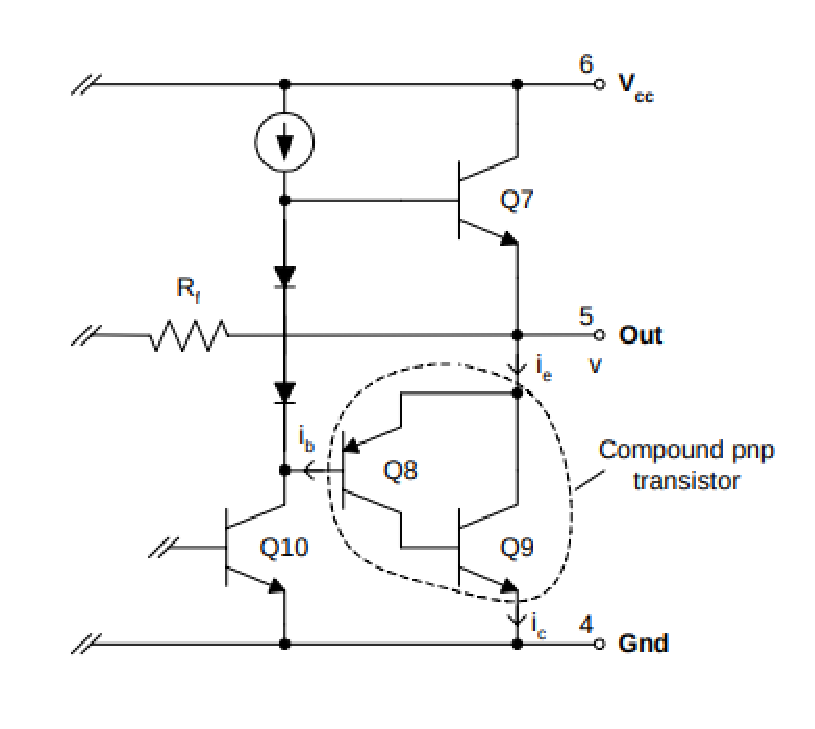
\includegraphics[width=0.4\textwidth]{./figs/LM3867.eps}
%
%\caption{}
%\label{fig:1}
%\end{figure}
\solution
Here,
$$\beta = \beta_{Q8} \beta_{Q9}$$  which is easy to show starting with
$i_{c8}=\beta_{Q8}i_{b8}$ and $i_{c9}=\beta_{Q9}i_{b9}$ . Compounding pnp’s was done in
early IC’s to improve the traditionally poor performance of pnp
transistors wrt frequency response, etc. 

\begin{figure}[!ht]
\centering	
\resizebox{\columnwidth}{!}{%\documentclass{article}
%\usepackage{tikz}
%\usepackage{circuitikz}
%\usepackage{amsmath}
%\usepackage{siunitx} % Preferred over SIunits
%
%\begin{document} 
%\begin{figure}
%
%
%\begin{center}
\begin{circuitikz}[scale=10]

\draw
(0,0) node[pnp] (pnp) {}
(pnp.base) to [short,i_=$i_b$,.-o] (-0.2,0)
(pnp.collector) to [short,i_=$i_c$,.-o] (0,-0.2)
(0,0.2) to [short,i_=$i_e$,o-.] (pnp.emitter)
(0,0) node[anchor = west] {$\beta\approx\beta_{Q9}\beta_{Q9}$}

;

\end{circuitikz}
%\end{center}
%\end{figure}
%\end{document}
}
\caption{Compound PNP}
\label{fig:compound}	
\end{figure}
%
%\begin{figure}[!ht]
%  \centering
% 
%    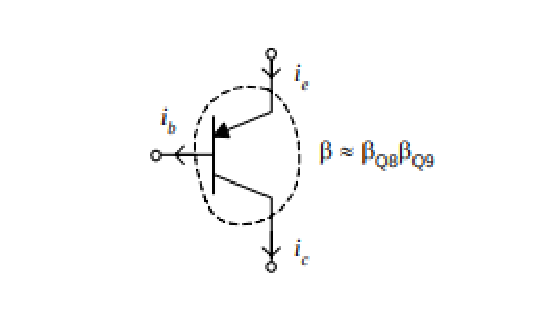
\includegraphics[width=0.5\textwidth]{./figs/LM3868.eps}
%
%\caption{}
%\label{fig:1}
%\end{figure}
\end{enumerate}

\section{Gain Calculation}
\begin{enumerate}[label=\thesection.\arabic*,ref=\thesection.\theenumi]
\item The class amplifier will amplify v such that we can assume $v>>v_{d}$. Derive the gain of the IC assuming the values of resistors given in the internal circuit.\\
\solution
\begin{figure}[!ht]
\centering	
\resizebox{\columnwidth}{!}{%\documentclass{article}
%
%\usepackage{tikz}
%\usepackage{circuitikz}
%\usepackage{siunitx}
%
%\begin{document}
%
%\begin{figure}
%  \begin{center}
    \begin{circuitikz}
      \draw (0,0)
      to[R=$\SI{15}{\kilo\ohm}$,-*] (0,2) % The voltage source
      to[R=$\SI{15}{\kilo\ohm}$,o-o]
      (0,4)node[anchor=south] {$V_{cc}$} 
      (0,2)to [short,o-o] (-1,2)node[anchor=east] {7}
      (4,-1) node[pnp] (pnp) {}
      (4,0)  [short,*-] to (pnp.E) 
      (pnp.E) node[anchor = north east] {$i$}
      (pnp.B) node[anchor = east] {$Q4$}
      (3.6,-1) node[anchor = east] {//}
      (4.4,-1.7) node[anchor = east] {//}
      
      (0.2,-0.2) -- (0.2,-0.3) -- (3.8,-0.3) --(3.8,-0.2)
      (2,-0.3) -- (2 , -0.5) node[anchor = north] {$R_e$}
      (0,-1) node[pnp] (pnp) {}
      (0,0)  [short,*-] to (pnp.E)
      (pnp.E) node[anchor = north east] {$i$}
      (pnp.B) node[anchor = east] {$Q3$}
      (-0.4,-1) node[anchor = east] {//}
      (0.4,-1.7) node[anchor = east] {//}
      (0,0) to[R={\SI{150}{\ohm}},-*] (2,0) to [R=$\SI{1.35}{\kilo\ohm}$,-*] (4,0) to[R={\SI{15}{\kilo\ohm}},-o]       node[pos=0.05,below left=1.5ex] {$R_f$}  (6,0) node[anchor = west] {$v$}
      (6,1.5) [->] node[anchor = south] {$Output$} -- (6,0.2)
      (4,0) [short,o-o] to (4,1.5)node[anchor = south] {$I$}
      (2,0) [short,o-o] to (2,1.5)node[anchor = south] {$8$};
      (4,-1) node[pnp] (pnp) {}
      (4,0)  [short,*-] to (pnp.E)

      
    \end{circuitikz}
   
%  \end{center}
%\end{figure}
%
%\end{document}
}
\caption{Amplifier Gain}
\label{fig:ampgain}	
\end{figure}
%\begin{figure}[!ht]
%  \centering
% 
%    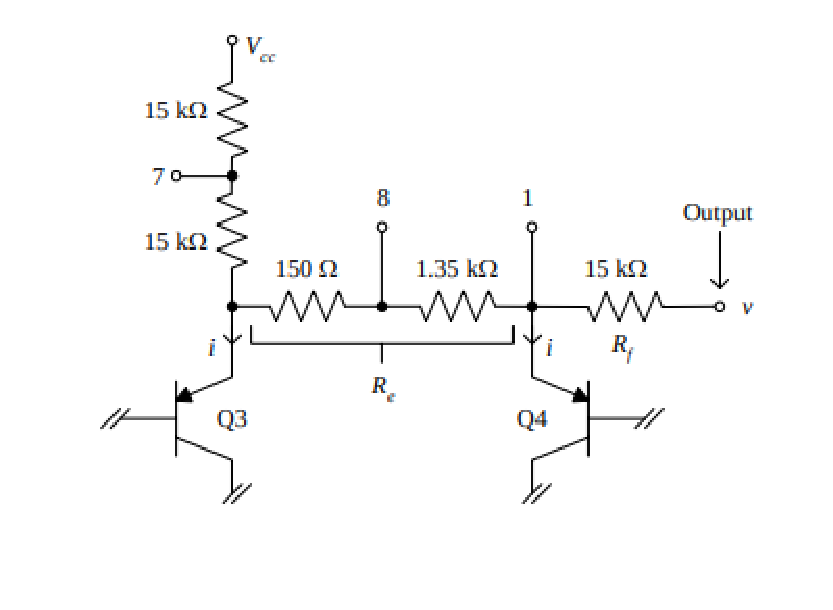
\includegraphics[width=0.5\textwidth]{./figs/LM3865.eps}
%
%\caption{}
%\label{fig:6}
%\end{figure}

After amplification by class AB amplifier,since we can assume $v>>v_{d}$ \\
Therefore , $$\frac{v}{R_{f}}=2i$$ \\
Also from small signal model we got,

   $$ \frac{v_{d}}{R_{e}}=2i
$$
From the above equations we get Gain, $$G=\frac{2 R_{f}}{R_{e}}$$\\
Substituting values from the IC we get $$G=\frac{2 \times 15k}{150+1350} =20$$    

\end{enumerate}
\end{document}
